\section{Experiment and Analysis}
\label{sec:experimentdesign}

To study spectrum utility in multiple area types, we develop experiments 
on off-the-shelf wireless platform and remote controlled spectrum analyzer measurement platform.
We do measurements in typical populated areas and sparse areas of DFW metropolitan carrying these platforms.
According to the measured data, we apply our Multiband Access Points Estimation framework to analyze
the performance of white space band application varying the population density.

\subsection{Experiment Design}
% Platform
To ensure the results are applicable, we employ a Linux-based 802.11 testbed~\cite{Gateworks}.
The platform includes a Gateworks 2358 board with Ubiquiti XR radios (XR9 at 900 MHz, 
XR2 at 2.4 GHz, XR5 at 5.2 GHz) and a DoodleLabs DL475 radio at 450 MHz~\cite{Ubnt,Gateworks}.
We developed shell script with tcpdump for this testbed working as a sniffer recording all 
802.11 packets.
The experiments taken in downtown Dallas, SMU campus, neighborhood show there is no 802.11
packets dected in white space bands. And in DFW area, as far as we know, we are the only 
group holds FCC license of white space bands. Our experiments verify that these bands 
have not been used for wireless data communication.
However, we observed that Gateworks platform only update its received signal strength when received
a new packet. It is not good for inter-network interference measurement. To cover the gap, 
we employ a spectrum analyzer, multiband antenna, mobile antenna and a laptop developing a spectrum sensing 
system. There is no mobile multiband antenna in market. We compare the multiband antenna measurement
and mobile antenna measurement across bands in lab with our controlled signal source.
Then normalize the received signal strength for mobile antenna measurement.

Our experiment platforms are shown in Figure~\ref{fig:equipment}.
  \begin{figure}
  %\vspace{-0.0in}
  \centering
  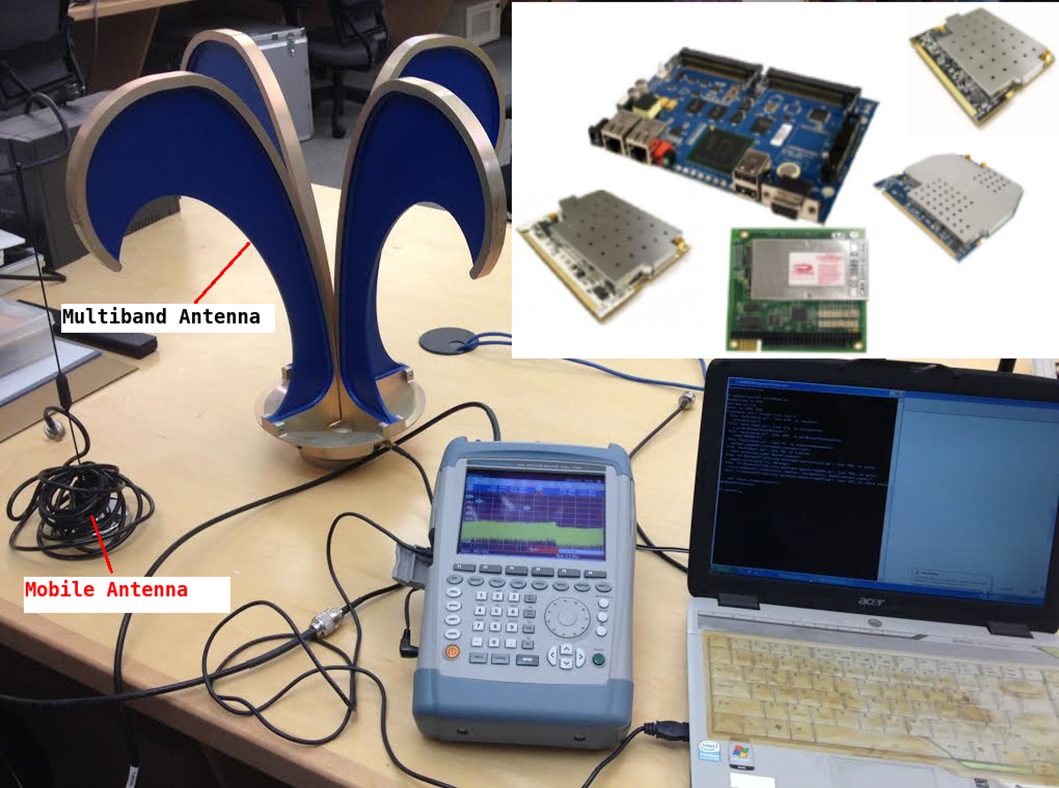
\includegraphics[width=74mm]{figures/equipment}
  \vspace{-0.1in}
  \caption{Multiband Measurement Platform}                                                                 
  \label{fig:equipment}
  %\vspace{-0.0in}
  \end{figure}
We has 32 samples each second from the spectrum analyzer system with time stamp of all bands.
Gateworks sniffer platform record all the packet received with time stamp. The duplicated 
samples are unique through the time stamp. Then we use the uniformed data for activity level
 calculation.  

% Location and Process 
%We apply drive test carrying our platform from Dallas to Weatherford as shown in~\ref{sec:problemformulation}.
We choose typical location according to population distribution and free white space bands 
from Google spectrum database~\cite{googledatabase}. The location chosen for experiments 
are Dallas, Weatherford and Millsap marked with stars in Figure~\ref{fig:drivemap}.
In Weatherford and Millsap, we monitor wireless activities in 3 location for 45 minutes in 
static on a normal weekday. The three locations of a city include downtown, neighborhood and 
rural area. In Dallas, we have multiple measurement in neighborhood, campus and sparse density area.
Then we post-process these data to get the activities level for each band in all the location.
Moreover, through our framework, the number for covering an arbitrary area is calculated and discussed in~\ref{subsec:result}.



\subsection{Results and Analysis} 
\label{subsec:result}

In table~\ref{tab:activitymeasurement}, we show our measurement results in multiple locations of DFW metro.
Dallas as the central city of North Texas, has the highest activities in most of the measured bands,
 especially in 450 MHz. The measurements of Dallas urban are taken from SMU campus, 2 neighborhoods
 and city Plano. We average these data finding 2.4 GHz is more active in urban area rather than 
 downtown area. Most of schools campus and neighborhoods are covered by public or private WiFi today,
which bring more activities in 2.4 GHz and 5.2 GHz.
In Weatherford, all the bands have less activities than Dallas. And due to the measurement location
we chosen, the rural area we chose on the west of Weatherford where could get more interference from
Fort Worth.
Millsap is a typical sparse city has 500 residents total in north Texas. The activities across all the bands are lower than
Dallas, and Weatherford. For 450 MHz, the activity reduce much faster than other bands in Dallas
and Weatherford. 

\begin{table*}
\centering % centering table 
\begin{tabular}{|l|c|c|c|c|c|c|c|c|c|c|c|} % creating 12 columns 
\hline %\hline % inserting double-line 
Bands     & \multicolumn{3}{c|}{Dallas} & \multicolumn{3}{c|}{Weatherford} & \multicolumn{3}{c|}{Millsap} \\% [0.5ex]
\hline % inserts single-line 
% Entering 1st row 
Area Type & Downtown & Urban & Sparse Area & Downtown &  Urban   & Sparse Area & Downtown & Urban & Sparse Area \\ % [0.5ex]
\hline % inserts single-line 
450 MHz &24.3667	&25.8274  &23.7667	&6.050 &12.50  &14.0333 & 7.0000 & 0.0667 & 0.0215 \\      
\hline % inserts single-line                                                                                                       
800 MHz &4.4000 	&16.4940  &4.7667	&5.2167&5.0667 &4.4333  & 3.8667 & 4.2000 & 3.6000 \\      
\hline % inserts single-line                                                                                                      
2.4 GHz &15.8667 	&34.9488  &2.6000	&2.0333&2.0333 &2.7667  & 2.0667 & 1.6000 & 0.8000 \\      
\hline % inserts single-line                                                                                                     
5.2 GHz &19.7000	&35.4571  &1.5333	&1.9333&1.9333 &1.3333  & 1.2667 & 2.0667 & 2.1000 \\      
\hline % inserts single-line 
\end{tabular}    
\label{tab:activitymeasurement}    
\caption{Activity Level in Multiple Locations} % title name of the table 
\vspace{-0.4in}
\end{table*}    

We put these measured activity level into our framework presented in~\ref{algorithm:mape}. We use Millsap
sparse area, Millsap downtown, Weatherford urban, Dallas rural and look up the population density on-line.
We input these information to our framework and calculate the number of access point for covering 
a $13 km \times 13 km$ area in different types. The output is shown in Figure~\ref{fig:redensity}. 

   \begin{figure}
   %\vspace{-0.0in}
   \centering
   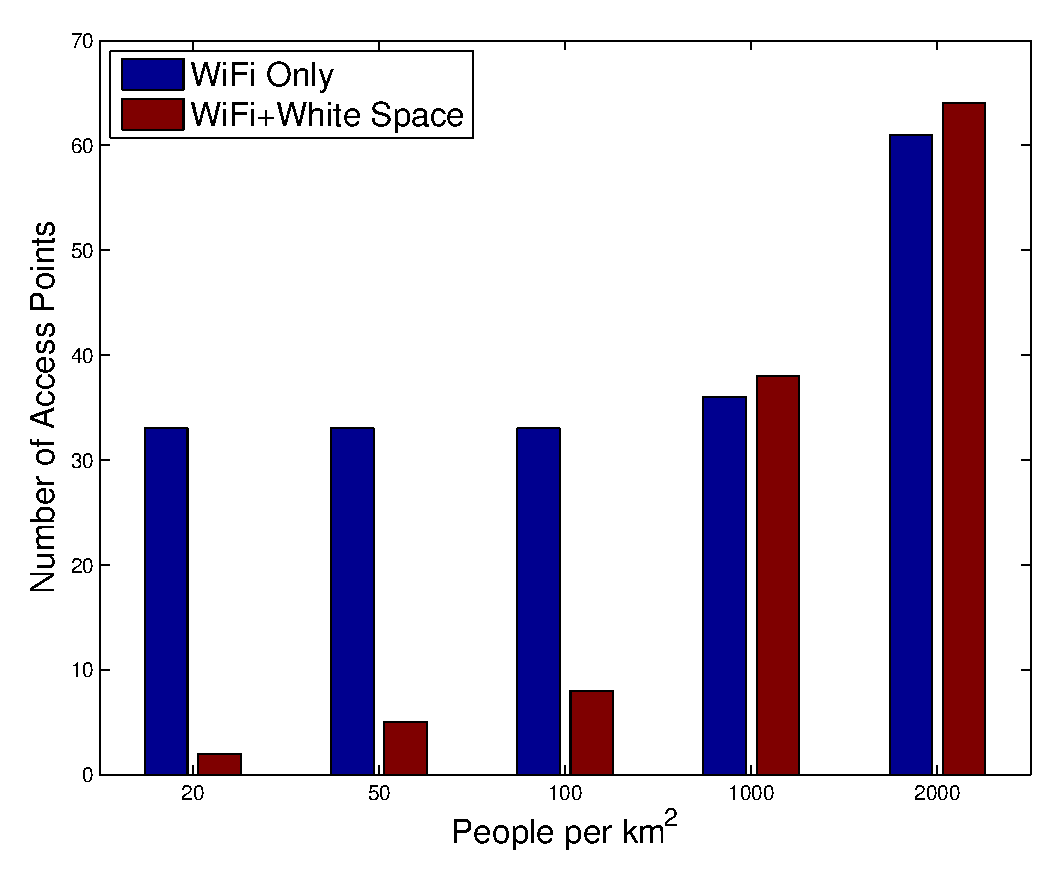
\includegraphics[width=74mm]{figures/redensity}
   \vspace{-0.1in}
   \caption{Number of Access Points need for 13x13 $km^2$ Area}                                                                 
   \label{fig:redensity}
   %\vspace{-0.0in}
   \end{figure}

% Experiment Results & expect results
We set the demand request as $2Mbps$ per person, the population
density as $20,50,100,1000,2000$ per square kilometers. We assume $30\%$ residents will use this
service. For WiFi only, we use 6 channels in 2.4 GHz, and 3 channels in 5.2 GHz. 
We adopt 802.11n maximum data rate 600 Mbps. For WiFi+ White Space
scenario, we use 3 channels in 450 MHz, 2.4 GHz and 5.2 GHz each. Then all the scenarios have the 
same channels in total. As shown in Figure~\ref{fig:redensity},
with the same number of channels, WiFi+White Space gains $1650\%$ comparing to WiFi only in 20 people 
per square kilometer scenario, and $660\%$ in 50 people per square kilometer and $412.5\%$ in 100 people
per square kilometer. But as the population density increase, due to the capacity constraint servicing
people in this area, low frequency white space band lose their advantage of larger communication range. 
And at the same time, the activities of other signal source, such as TV station in downtown area reduce
the capacity of white space band, then WiFi+White Space bands perform worse than WiFi only bands combination.
Moreover, if we count the intra-network interference, the situation could be even worse.


To find the best bands combination, we select 500 people per square kilometer scenario and use Weatherford 
downtown spectrum to calculate the number of access points in this area. We assume the total number of channels 
is 12. The other setup of the experiment is 
the same as the previous configuration. The results are shown in~\ref{fig:varybandcomb}.
   \begin{figure}
   %\vspace{-0.0in}
   \centering
   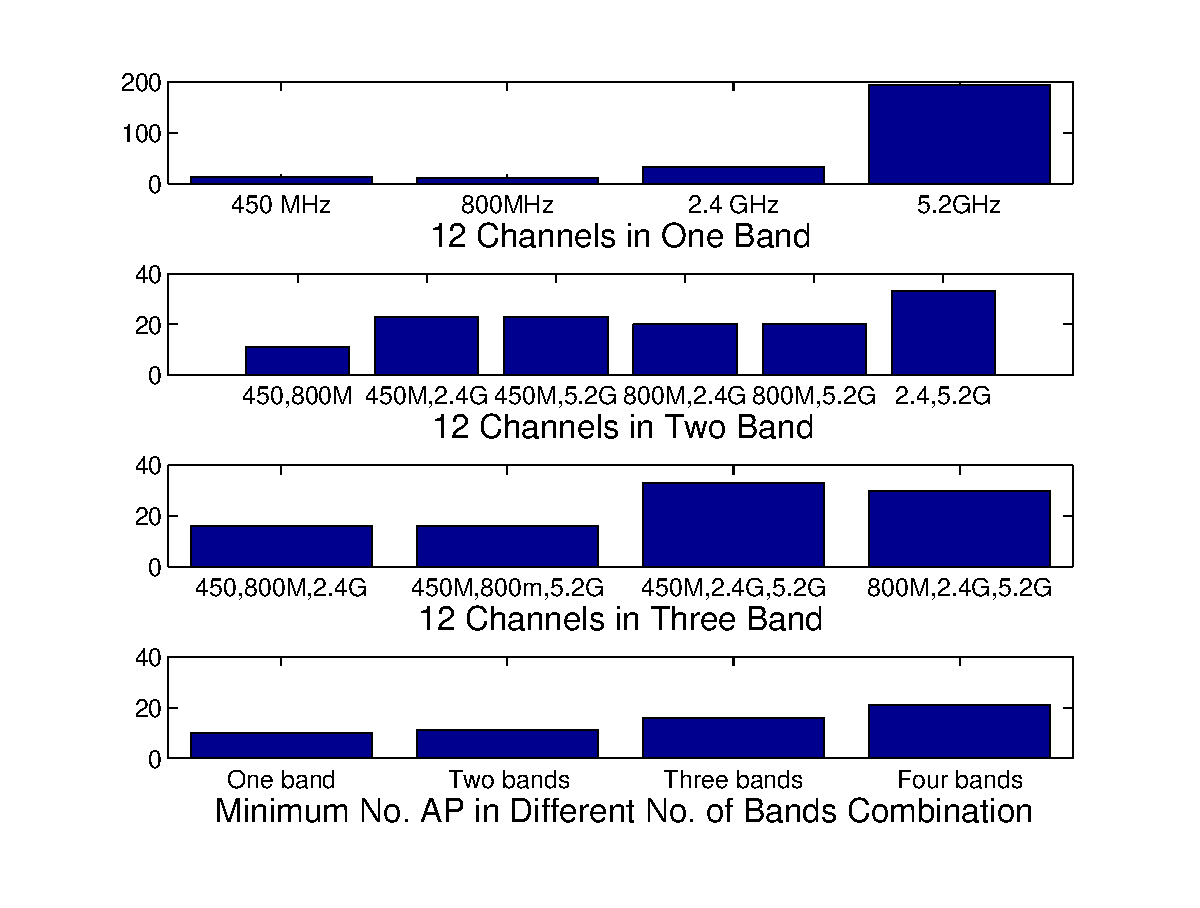
\includegraphics[width=94mm]{figures/varybandcomb}
   \vspace{-0.1in}
   \caption{Bands Combinations of The Same No. of Channels in 500 Population Density}                                                                 
   \label{fig:varybandcomb}
   %\vspace{-0.0in}
   \end{figure}

The first subplot in the Figure is the number of access points needs for 12 channels in one band.
As frequency goes up, more access points need to serve this area. 450 MHz does not outperform 
800 MHz since in this population density, they have the same service area.
Subplot 2 shows if we have equal channels in 2 bands, white space bands combination performs better
than WiFi by 63.64\% and WiFi + white space bands by 56.52\%. In this scenario, the more white space bands channels are 
used, the better performance will be got.

   \begin{figure}
   %\vspace{-0.0in}
   \centering
   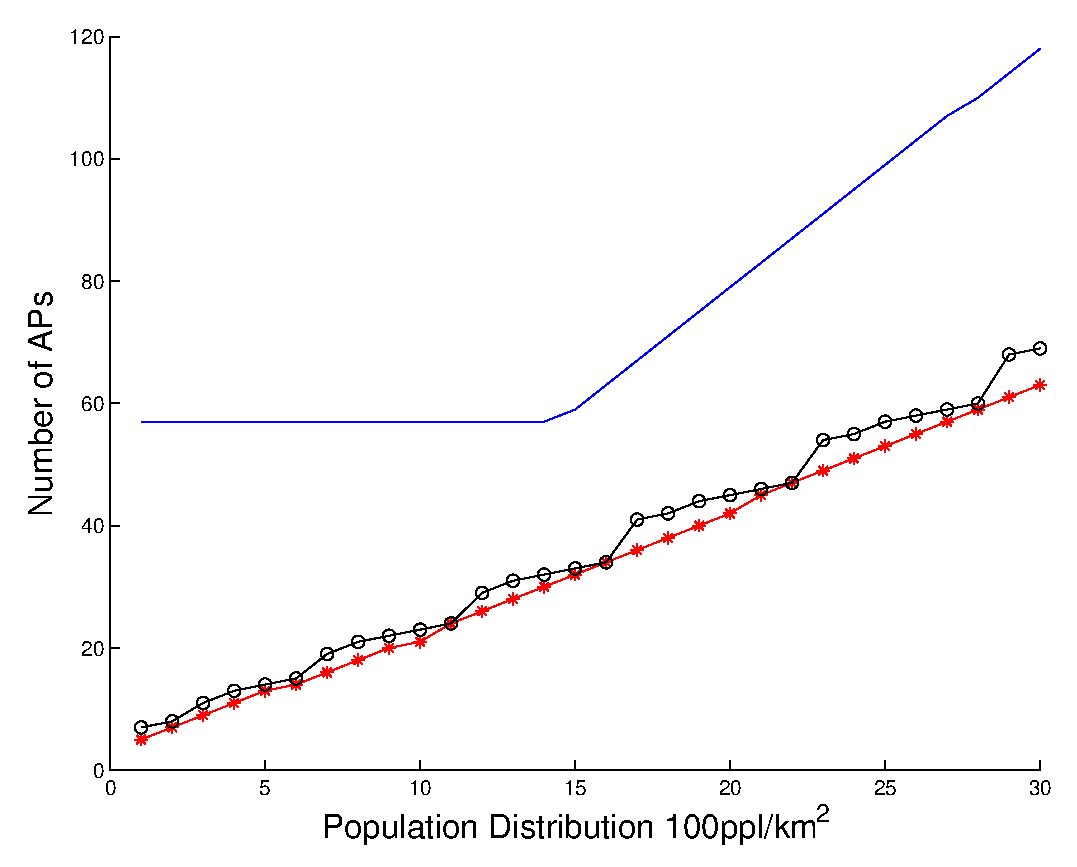
\includegraphics[width=94mm]{figures/varybandcomb2}
   \vspace{-0.1in}
   \caption{Bands Combinations of The Same No. of Channels in 1500 Population} 
   \label{fig:varybandcomb2}
   %\vspace{-0.0in}
   \end{figure}

We reset the population as 1500. And Dallas urban spectrum activity is used in\ref{fig:varybandcomb2}.
In this scenario, using all channels in white space band has the same performance comparing to WiFi+
White space bands. And generally white space band still have benefit reducing the number of access points
by 23.33\% and 9.19\%. As population density increase, the gain brought by white space decrease. The best
band combination is still the combination with white space bands. 

